\subsection{Unrolling Results}
\begin{figure}[h]
\centering
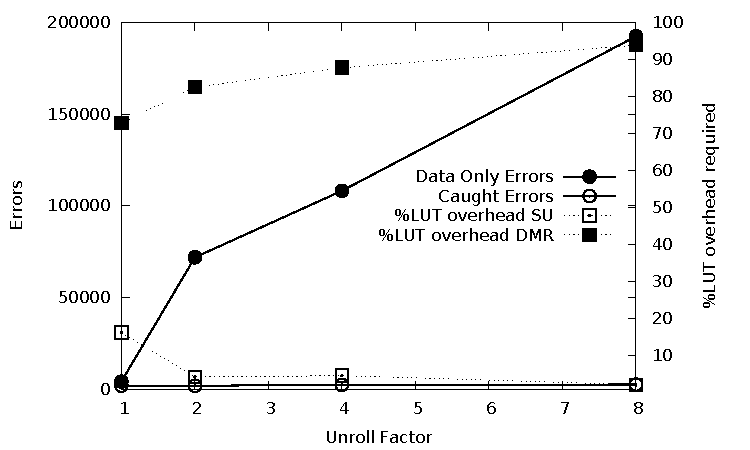
\includegraphics[width=3.5in]{./graphs/dp_unrolling_res.pdf}
\caption{Data Only Errors and Caught Errors for a dot product loop unrolling with StitchUp along with \%LUT overhead against DMR}
\label{fig:dp_unrolling_res}
\end{figure}


\subsection{Resource Overheads}
\renewcommand{\arraystretch}{0.8}
\begin{table*}[t]
\small
\singlespace
\centering
\caption{Resource Usage Results}
\label{tab:resources}
\tabcolsep=0.11cm
\begin{tabular}{@{}|l|l|l|l|l|l|l|l|l|l|l|l|l|@{}}
\toprule
                    & \multicolumn{4}{l|}{\textbf{Original}}                      & \multicolumn{4}{l|}{\textbf{StitchUp}}                      & \multicolumn{4}{l|}{\textbf{DMR}}                           \\ \midrule
\textbf{Bench}      & \textit{LUT} & \textit{REG} & \textit{DSP} & \textit{Pow}   & \textit{LUT} & \textit{REG} & \textit{DSP} & \textit{Pow}   & \textit{LUT} & \textit{REG} & \textit{DSP} & \textit{Pow}   \\ \midrule
\textit{aes}        & 47230        & 28152        & 0            & 299.346        & 47539        & 28800        & 0            & 316.186        & 90467        & 53944        & 0            & -              \\ \midrule
\textit{adpcm}      & 21050        & 16752        & 168          & 133.962        & 29599        & 29484        & 178          & 156.903        & 38664        & 31077        & 348          & -              \\ \midrule
\textit{blowfish}   & 97002        & 45320        & 0            & -              & 97440        & 46039        & 0            & -              & 194598       & 88268        & 0            & -              \\ \midrule
\textit{dfadd}      & 4639         & 4310         & 0            & 50.0916        & 5562         & 5095         & 0            & 54.224         & 6394         & 5754         & 0            & 58.114         \\ \midrule
\textit{dfdiv}      & 12144        & 13157        & 30           & 100.435        & 22254        & 23449        & 60           & 145.577        & 22811        & 23904        & 60           & 147.027        \\ \midrule
\textit{dfmul}      & 3348         & 3912         & 16           & 47.024         & 4553         & 4845         & 32           & 54.128         & 5105         & 5397         & 32           & 57.521         \\ \midrule
\textit{dfsin}      & 21343        & 20347        & 71           & 137.802        & 40928        & 38116        & 136          & 222.217        & 41136        & 38321        & 142          & -              \\ \midrule
\textit{gsm}        & 11953        & 9879         & 72           & 147.006        & 22049        & 17228        & 144          & 260.730        & 22399        & 17331        & 144          & 265.949        \\ \midrule
\textit{mips}       & 8278         & 6367         & 4            & 89.326         & 15639        & 10231        & 8            & 132.409        & 14304        & 10351        & 8            & 134.316        \\ \midrule
\textit{motion}     & 52665        & 26743        & 1            & -              & 104840       & 50719        & 1            & -              & 106986       & 51199        & 2            & -              \\ \midrule
\textit{sha}        & 9117         & 9287         & 3            & -              & 9491         & 10188        & 6            & -              & 16788        & 16189        & 6            & -               \\ \bottomrule
\end{tabular}
\end{table*}

%Power Results
\subsection{Power Results}
\begin{figure}[h]
\centering
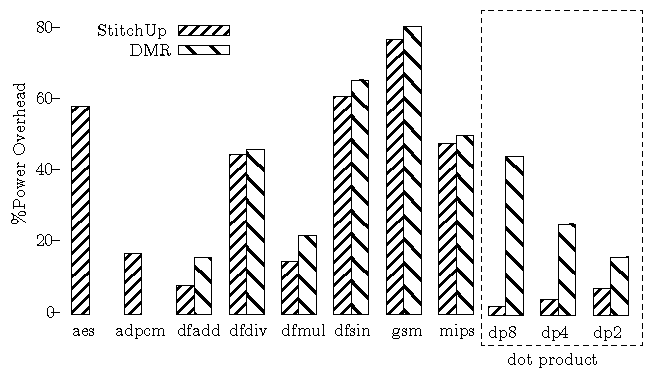
\includegraphics[width=3.5in]{./graphs/power_results.pdf}
\caption{Comparison of \% power overheads required for both StitchUp and DMR}
\label{fig:power_res}
\end{figure}

\begin{figure}[h]
\centering
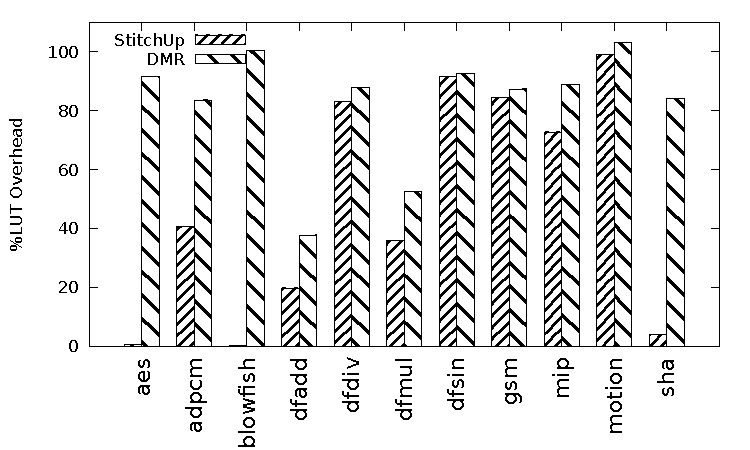
\includegraphics[width=3.5in]{./graphs/luts_res.pdf}
\caption{Comparison of \% LUT overheads required for both StitchUp and DMR}
\label{fig:lut_res}
\end{figure}

\subsection{Fault Injection Results}

\begin{figure}[h]
\centering
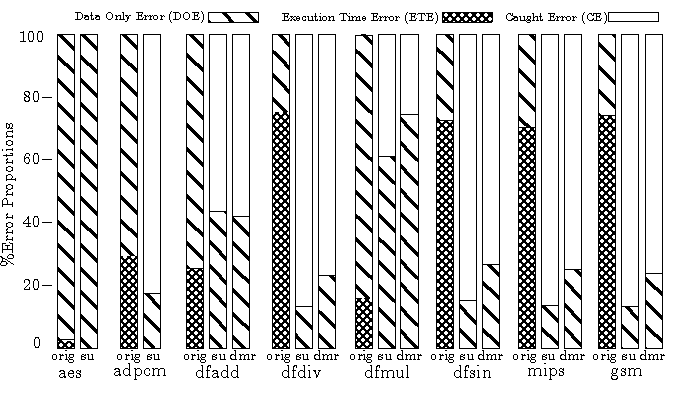
\includegraphics[width=3.5in]{./graphs/errors_res.pdf}
\caption{Error results for the CHStone benchmarks}
\label{fig:error_res}
\end{figure}


%\begin{table*}[t]
%\small
%\singlespace
%\centering
%\caption{Fault Injection Results}
%\label{tab:faults}
%\tabcolsep=0.11cm
%\begin{tabular}{|l|l|l|l|l|l|l|l|l|l|}
%\hline
%                    & \multicolumn{3}{l|}{\textbf{Original}} & \multicolumn{3}{l|}{\textbf{StitchUp}} & \multicolumn{3}{l|}{\textbf{DMR}} \\ \hline
%\textbf{Benchmarks} & \%ETE       & \%DOE       & \%CE       & \%ETE       & \%DOE       & \%CE       & \%ETE      & \%DOE     & \%CE     \\ \hline
%\textit{aes}        &             &             &            &             &             &            &            &           &          \\ \hline
%\textit{adpcm}      &             &             &            &             &             &            &            &           &          \\ \hline
%\textit{dfadd}      &             &             &            &             &             &            &            &           &          \\ \hline
%\textit{dfdiv}      &             &             &            &             &             &            &            &           &          \\ \hline
%\textit{dfmul}      &             &             &            &             &             &            &            &           &          \\ \hline
%\textit{dfsin}      &             &             &            &             &             &            &            &           &          \\ \hline
%\textit{gsm}        &             &             &            &             &             &            &            &           &          \\ \hline
%\textit{mips}       &             &             &            &             &             &            &            &           &          \\ \hline
%\textit{sha}        &             &             &            &             &             &            &            &           &          \\ \hline
%\end{tabular}
%\end{table*}

